\section{Design}
\label{s:design}

\subsection{Design Goals}
\label{subsec:design-goals}

\sys components are designed with the
general goal of
allowing for the assembly
of a wide variety of in situ workflows.
Below are some general guidelines
for the design of such components
which both guided the design of the existing \sys
components and which we also gained in retrospect.

1) To allow for the greatest variety of workflows,
data manipulation primitives and data analysis components
should be packaged in similar ways -- that is,
regardless of their individual complexity,
the pieces that make up these workflows
should export compatible interfaces as much as possible.

2) The ability to handle multi-dimensional data,
along with the consistent labeling of
dimensions and quantities as meta-data,
allows for components that are highly
adaptable and simple to use. By designing components
that can operate, as much as possible, on data
having any number of dimensions, we can
allow for a large variety of arrangements
of components.

3) While different types of components understand
varying levels of semantics, maintaining a
high level of semantics (i.e., labeling
quantities and dimensions as much
as possible) early on and when passing
through components that do not necessarily
require all of these labels allows for the most
functionality downstream.

4) Because programming languages understand
multi-dimensional data as being in a
specific order in memory, there is a need for
components that re-arrange data and
re-label its dimensions without necessarily
changing its size. Indeed, when data is stored
in a database on disk, it is simple to gain a desired
view of the data, for example by using SQL.
However, in the middle of a real-time workflow,
data must be presented to the components in a
format that they expect and understand.
This requires a specific ordering of data in
memory.
We expand on this topic in the description
of the Dim-Reduce component later in this section.
%in~\autoref{subsec:dimreduce}.

These insights guide the design for the
reusable workflow components presented in this
paper. From a general perspective, designing a smaller number of
components to assemble workflows with finer step decomposition
allows for more general processing
than designing more numerous components each having more
complex functionality.
And, as we show in~\autoref{s:eval}, componentizing
the analysis involves only minor changes
in overall workflow performance.

\subsection{Components Overview}

\sys currently consists of four generic components
that perform common operations
in scientific workflows. These are Select,
Magnitude, Dim-Reduce, and Histogram.
Again, the choice of these components
is not meant to encompass as wide a variety
of workflow purposes as possible as-is.
However, that we were able to deploy three
very different workflows driven by different
scientific codes using the existing \sys
components demonstrates a promising approach.

Each component is a single MPI executable
that uses the self-describing property
of data exchanged through ADIOS
to discover the dimensions and their sizes of
the data it receives from its upstream component;
in this way, the component is able to
automatically partition the generally
large dataset that it receives
among its constituent processes.
The component in question
then operates on the data
in a way that is specified by the user
through command-line parameters.
By specifying the names of the streams
and the arrays that hold the data
of interest through additional parameters, the
user is able to specify an entire
workflow as a series of 
applications launched together in a single
job script.
This procedure is detailed in~\autoref{s:eval}.

Finally, the components are designed
based on the assumption that the driving simulation
outputs data at regular time steps.
When it is done processing the data belonging
to a particular time step for a stream, a component
can request the data in the next time step.
With FlexPath, this works as follows:
readers block until
the corresponding writers
are ready to output the data;
similarly, until readers are able to
request the data for the next time step,
corresponding writers store the data for
this step in an internal queue.

\subsection{Select}

\begin{figure}
  \begin{lstlisting}
    aprun select _input-stream-name_ _input-array-name_ _dimension-index_ _output-stream-name_ _output-array-name_ [_arg1_] [_arg2_] (*@\ldots@*)
  \end{lstlisting}
%  \vspace{-0.15in}
  \caption{Select Component Usage}
  \label{fig:select}
%  \vspace{-0.10in}
\end{figure}

Given an input stream that includes an array with
any number of dimensions,
the Select component extracts certain rows (indices) from one of
the dimensions.
Thus, it outputs an array
with the same number of dimensions,
but with the dimension of interest having a
smaller size. In order to select the quantities of
interest, the component uses a header which
must be passed by the previous component in the
workflow as part of the meta-data that ADIOS
can include in the stream.
The header is a list of strings that
name the quantities in the
dimension of interest.
This allows the user the specify
the names of the quantities (rows)
to select by name, rather than by index number,
which is easier to do when preparing the launch script.

~\autoref{fig:select} illustrates the usage
of the Select component. 
The input and output stream and array names
identify the stream and dataset on
which Select operates, as well as how
the component renames them in its output.
All components use similar parameters; this lets
the user assemble a workflow by
using the same stream and array names
for the output of an upstream component
as for the input of its downstream component.

The parameter \texttt{dimension-index} identifies
the dimension in which Select will filter
certain rows. ADIOS maintains the number of dimensions
as meta-data in the stream, and one can identify them
by number. Finally, the \texttt{arg1} \ldots \ parameters 
identify the names of the rows to keep in the dimension
of interest. Select is able identify these rows
by name using the header described previously.

\subsection{Magnitude}

The Magnitude component calculates the magnitudes
of an array of vectors. That is, it operates
on a two-dimensional array, where one dimension spans
the data points, for example the particles that
make up a simulation, and the other dimension spans any number
of components of the same vector for each data point, for example
the three-dimensional components of velocity,
as we use it in one workflow we demonstrate later.

The output of Magnitude is a one-dimensional array holding
the magnitudes of the input vectors. This \sys component
only takes the names of the input and output streams
as command-line parameters, since it always
operates on a two-dimensional array.

\subsection{Histogram}

\begin{figure}
  \begin{lstlisting}
    aprun histogram _input-stream-name_ _input-array-name_ _num-bins_
  \end{lstlisting}
%  \vspace{-0.15in}
  \caption{Histogram Component Usage}
  \label{fig:histogram}
%  \vspace{-0.10in}
\end{figure}

The processes that make up the Histogram component
partition among themselves a one-dimensional
array of data. They communicate to discover the global
minimum and maximum values in the array, create a
number of bins between these two extremes, and
then communicate again to count the number of values in the
globally partitioned array that fall in each bin.
The number of bins to use must be passed to the
component when it is launched.

In our current implementation, one of the processes
of Histogram writes the
output to a file on disk. We chose this approach
because this component is often used as an
endpoint in the workflow and because the output of this
component is generally very small compared to its input
and can be easily written by a single process.

~\autoref{fig:histogram} illustrate the usage of
the Histogram component. Because it is currently
implemented as an endpoint component, Histogram
only requires the names of the \textit{input}
stream and array names. In addition, the user
specifies the desired number of bins.

\subsection{Dim-Reduce}

\begin{figure}
  \begin{lstlisting}
    aprun dim-reduce _input-stream-name_ _input-array-name_ _dim-to-remove_ _dim-to-grow_ _output-stream-name_ _output-array-name_
  \end{lstlisting}
%  \vspace{-0.15in}
  \caption{Dim-Reduce Component Usage}
  \label{fig:dim-reduce}
%  \vspace{-0.10in}
\end{figure}

\begin{figure}
  \centering
  \vspace{-0.10in}
  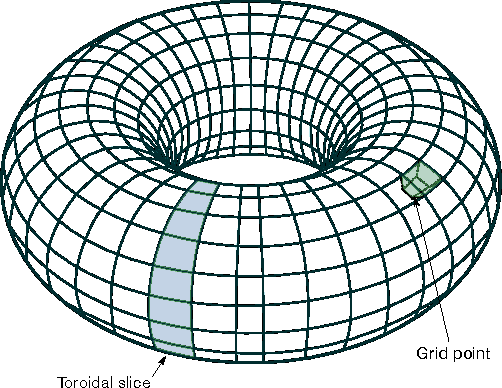
\includegraphics[width=0.7\columnwidth]{fig/Simple_Torus_mod}
  \vspace{-0.09in}
  \caption{Representation of GTCP Toroid, modification of \cite{WikimediaCommons:torus}}
  \label{fig:toroid}
  \vspace{-0.20in}
\end{figure}


Dim-Reduce is a component that removes one dimension from its
input array, ``absorbing'' it into another dimension without
modifying the total size of the data.

This operation is necessary because certain analytical
components in workflows expect data having a particular number
of dimensions.
Due to the fact that  multi-dimensional data is arranged
in a particular order in memory, this operation
can require a re-arrangement
of the data in the overall linear representation
of the multi-dimensional array.

To better explain the need for Dim-Reduce, we turn to one
workflow which we explain in more detail later.
GTCP is a toroidal plasma simulator,
which breaks up the plasma into toroidal slices and grid points,
each having a number of associated physical quantities
that describe it (such as the pressure inside it), as illustrated
in~\autoref{fig:toroid}.

In the workflow that is driven
by this simulation, we wish to obtain
as a final result a histogram of
all the pressures at all grid points
in the entire toroid.
However, the Histogram component expects
one-dimensional data. As it is output
from the GTCP simulation, the data is
three-dimensional, with one dimension
spanning the \textit{toroidal slices}
of the toroid, another dimension
spanning the \textit{grid points} inside of each such
slice, and the last dimension spanning the
7 quantities that describe
various \textit{properties} of the plasma
in each grid point.

To turn this three-dimensional data
into a format that Histogram can operate
on, the data must pass through two instances
of Dim-Reduce. We describe the workflows
in greater detail in~\autoref{s:eval}.


\if 0
In this section, we first present
some insights in the design of
generic workflow components,
and we then discuss
some of our implementation choices
and how they allowed us to 
build these components.

\subsection{Insights: Overview}

By evaluating the presented workflows
and considering other workflows with
which the authors are familiar,
four key insights are revealed.

1) To allow for the greatest variety of workflows,
data manipulation primitives and data analysis components
should be packaged in similar ways -- that is,
regardless of their individual complexity,
the pieces that make up these workflows
should export compatible interfaces as much as possible.

2) The ability to handle multi-dimensional data,
along with the consistent labeling of
dimensions and quantities as meta-data,
allows for components that are highly
adaptable and simple to use.

3) While different types of components understand
varying levels of semantics, maintaining a
high level of semantics (i.e., labeling
quantities and dimensions as much
as possible) early on and when passing
through components that do not necessarily
require all of these labels allows for the most
functionality downstream.

4) Because programming languages understand
multi-dimensional data as being in a
specific order in memory, there is a need for
glue components that re-arrange data and
re-label its dimensions without necessarily
changing its size. Indeed, when data is stored
in a database on disk, it is simple to gain a desired
view of the data, for example by using SQL.
However, in the middle of a real-time workflow,
data must be presented to the components in a
format that they expect and understand.
This requires a specific ordering of data in
memory. We expand on this topic in~\autoref{subsec:dimreduce}.

These insights guide the design for the
reusable glue and analysis
components presented in this
paper. From a general perspective, designing a smaller number of
components to assemble workflows with finer step decomposition
allows for more general processing
than designing more numerous components each having more
complex functionality.
And, as we show in~\autoref{s:eval}, componentizing
the analysis involves only minor changes
in overall workflow performance.

\subsection{Multi-Dimensional Data Support}

Many scientific codes serialize their output, effectively packing
multi-dimensional data into a single dimension.
However, this technique offers
little information on the data to downstream
components in a workflow.

For example, two of the simulations used in the
workflows presented in this work inherently
pack their output into one-dimensional arrays
for native output, even
though LAMMPS' output is logically
two-dimensional and that
of GTCP three-dimensional.
In order to use the same glue code to
extract desired data from both outputs,
this code must be able to operate on two-dimensional data
as well as three-dimensional data.
In fact, if the glue code is able to operate
on any number of dimensions, all that must be provided to it
at runtime is the dimensions and indices to extract.
This is precisely the role of our
{\em Select} component.

In general, it is advantageous to (1) design
components that can operate on
multi-dimensional data as much as possible
and (2) format the output data of
scientific applications as having well-defined
dimensions. Emphasizing the support for multi-dimensional
data in the design of workflow components allows
for maximum compatibility between the interfaces
of components by providing a
consistent way to refer to the data.

Still, while multi-dimensional data support
provides a consistent way to refer
to the data, not all components should be
designed so as to work with
any number of dimensions.
For example, we found it advantageous to
design our {\em Histogram} component to work with
only one dimension since this is
a natural input for a histogram operation.

\if 0
Indeed, creating a histogram from one-dimensional data is intuitive.
Supporting a higher number of dimensions
would add unnecessary complexity
to this component. If the data has more
dimensions than are expected,
and only particular indices in a particular
dimension hold the data of interest,
we can simply use filter and selector
glue to extract and format the data for
{\em Histogram} to operate on.
\fi

\subsection{Semantics}

When data is organized under clearly defined
dimensions, labeling these
dimensions and the indices they hold
as the data goes through each component
lets downstream subscribers
refer to dimensions using their names.
Because the data is potentially re-sized
and re-arranged in the course of a workflow,
it is useful to maintain such
semantics as much as possible. However,
the absence of labels should not block
the workflow execution.

For example, in both the LAMMPS and the GTCP workflows, we modified
the simulations so that they label the
quantities that they output in the
dimension that holds
these quantities. This lets the Select component
extract the quantities of interest by referring
to them by name. However, we did not label the dimensions
themselves, rather referring to them by number. 

When they exist, these labels are concatenated
into a header string passed along to the
next component in the workflow as another variable
through the ADIOS interface, alongside the main
simulation data.
While in our current implementation, Select is hard-coded to
always looks for such a header describing the quantities
in the dimension of interest, 
we can easily extend this functionality to let the user either refer
to dimensions and indices by name, when headers exist, or by number,
when they do not.

In general, labels should be used as much as possible, but they
should also be kept optional.

\subsection{Dimension Reduction}
\label{subsec:dimreduce}
As discussed earlier, there is a need in
scientific workflows with fine
step granularity for glue components
that re-arrange and re-label data
without necessarily changing its size.
This is illustrated by the need for the {\em Dim-Reduce}
operation in the GTCP workflow.

In its raw output, GTCP keeps track of the
toroidal slice that produces the data of interest by using a
dimension that spans the ``Toroidal rank'' of grid points.
In our workflow, we
wish to create histograms encompassing all grid
points in the toroid, thereby
eliminating the concept of ``Toroidal rank''
along the way
and instead growing the dimension
that spans the number of grid points.

Programming languages represent multi-dimensional
arrays in a specific order in
memory, so we cannot simply keep the data
ordered as it is, change the number
of dimensions and their sizes as ADIOS understands them, 
and assume that the new dimensions correctly
reference the data.

The dimensions of GTCP's raw output are 
$N_0{\times}N_1{\times}N_2$, where:

\begin{itemize}

\item $N_0$ is the size of the {\em toroidal rank} dimension $D_0$

\item $N_1$ is the size of the {\em gridpoint} dimension $D_1$

\item $N_2$ is the size of the {\em property} dimension $D_2$

\end{itemize}

At one stage of the GTCP workflow, we wish
to eliminate the concept of
{\em toroidal rank} of the data. This is to bring the data one step
closer to a format that Histogram understands:
one-dimensional data.
For the data to be one-dimensional, two instances of the
Dim-Reduce operation are required.
We focus here on the first of the two.

The desired result of this operation is that:

\begin{itemize}

\item The concept of {\em toroidal rank} of a particle disappears.

\item The concept of {\em gridpoint number} loses its
  original meaning and takes
  on a new one; the indices in this dimension now
  cover all gridpoints in the toroid,
  rather than only those in a particular toroidal slice.
  
\item The concept of {\em property} keeps its original
  meaning, and the size of its dimension is unchanged.

\end{itemize}

We can say that $D_1$, the {\em gridpoint} dimension,
\textbf{\em absorbs} $D_0$, the {\em toroidal rank} dimension.
The array resulting from this
operation has dimensions $N_1'{\times}N_2$ , where:

\begin{itemize}

\item $N_1' = N_0{\times}N_1$ is the new {\em gridpoint} dimension $D_1'$ size

\item $N_2' = N_2$ is the {\em property} dimension $D_2'$ size

\end{itemize}

We call this operation {\em dimension reduction}.
Even though it does not
change the size of the data set, we have seen in our implementation 
that it often changes the in-memory
ordering of data. Consequently, it is still potentially a
compute-intensive operation with sizable communication overhead
when the dataset is large and many
processes are involved in it.

This operation fits well into a
SuperGlue component, and it is precisely
the role of the Dim-Reduce
component, which can operate on a dataset having
any number of dimensions.

\subsection{Implementation Artifacts}

Though we refer to the SuperGlue components as single entities,
they are distributed
codes able to split computation on large dataset
among the processes of which they are
composed. More precisely, they are MPI executables written in C
where all processes in a component belong to the
same MPI communicator.

To connect components, we use
ADIOS~\cite{lofstead:2009:adaptable}
for the flexibility in writing destinations,
reading sources, and offering a
typed data stream. In particular, we use
the FlexPath transport. It implements
a {\em stream-based} data exchange abstracted to
the components through the
ADIOS interface, is asynchronous, and allows for
data exchange between any
number of writers and readers. Therefore:

1. We can launch components of the workflow
in any order: downstream components
will wait for the availability of data from
upstream components and upstream
components will buffer data up to a certain
size until they are able to send it
downstream. In our experiments,
we launch all components simultaneously.

\if 0
This also means that the decision as to
which downstream components to use can be made after
the upstream components have started
running allowing for real-time adjustments to the
workflow based on results obtained upstream.
\fi

2. Even if the number of processes used for one
component is different from that used for the previous
one in the workflow, each component can split the data
(and therefore the computation) evenly among its processes.

3. A FlexPath stream actually corresponds
to the internal buffering of data on the writer side
until readers are ready to request the data,
at which point the data exchange
on the writer side is carried out
by a separate thread.
This asynchronous communication allows a 
SuperGlue component to move on to the computation
of a subsequent timestep even when a downstream
component is not yet ready to accept data,
effectively overlapping computation and IO
and offering high performance to a componentized workflow.

\if 0
We should mention, however, due to the current implementation of FlexPath, there is overhead
data exchanged when different numbers of writers and readers are used. Even if
reader $R$ requests only a portion of writer $W$'s data, the current implementation
is such that $W$ sends all of its data to $R$. This is in the process of being
improved, and this effort is orthogonal to the work done for this project.
\fi

ADIOS and its transports, such as FlexPath,
keep track of the
data dimensions and their sizes. Therefore, when a
component receives a
multi-dimensional array, it can discover the dimensions
of the data and their
sizes as defined by the previous component
in the workflow and divide the global array
and split the computation accordingly.

There is no need to re-compile SuperGlue components when using them
in different workflows. Any configuration
of a component for a particular workflow
can be provided through run-time arguments.
We will show more clearly how this is done in the next section,
but in general, the user must specify the
stream and array names from which to read
and to which to write,
and usually also dimensions and/or
indices to operate on.
Referring to
streams and arrays using names allows users to
easily chain together these
components into potentially complex workflows.

\fi
